\documentclass{beamer}
\mode<presentation>
\usepackage{amsmath}
\usepackage{amssymb}
%\usepackage{advdate}
\usepackage{adjustbox}
\usepackage{subcaption}
\usepackage{enumitem}
\usepackage{multicol}
\usepackage{mathtools}
\usepackage{listings}
\usepackage{url}
\def\UrlBreaks{\do\/\do-}
\usetheme{AnnArbor}
%\usecolortheme{lily}
\setbeamertemplate{footline}
{
	\leavevmode%
	\hbox{%
		\begin{beamercolorbox}[wd=\paperwidth,ht=2.25ex,dp=1ex,right]{author in head/foot}%
			\insertframenumber{} / \inserttotalframenumber\hspace*{2ex} 
		\end{beamercolorbox}}%
		\vskip0pt%
	}
	\setbeamertemplate{navigation symbols}{}

	\providecommand{\nCr}[2]{\,^{#1}C_{#2}} % nCr
	\providecommand{\nPr}[2]{\,^{#1}P_{#2}} % nPr
	\providecommand{\mbf}{\mathbf}
	\providecommand{\pr}[1]{\ensuremath{\Pr\left(#1\right)}}
	\providecommand{\qfunc}[1]{\ensuremath{Q\left(#1\right)}}
	\providecommand{\sbrak}[1]{\ensuremath{{}\left[#1\right]}}
	\providecommand{\lsbrak}[1]{\ensuremath{{}\left[#1\right.}}
	\providecommand{\rsbrak}[1]{\ensuremath{{}\left.#1\right]}}
	\providecommand{\brak}[1]{\ensuremath{\left(#1\right)}}
	\providecommand{\lbrak}[1]{\ensuremath{\left(#1\right.}}
	\providecommand{\rbrak}[1]{\ensuremath{\left.#1\right)}}
	\providecommand{\cbrak}[1]{\ensuremath{\left\{#1\right\}}}
	\providecommand{\lcbrak}[1]{\ensuremath{\left\{#1\right.}}
	\providecommand{\rcbrak}[1]{\ensuremath{\left.#1\right\}}}
	\theoremstyle{remark}
	\newtheorem{rem}{Remark}
	\newcommand{\sgn}{\mathop{\mathrm{sgn}}}
	\providecommand{\abs}[1]{\left\vert#1\right\vert}
	\providecommand{\res}[1]{\Res\displaylimits_{#1}} 
	\providecommand{\norm}[1]{\lVert#1\rVert}
	\providecommand{\mtx}[1]{\mathbf{#1}}
	\providecommand{\mean}[1]{E\left[ #1 \right]}
	\providecommand{\fourier}{\overset{\mathcal{F}}{ \rightleftharpoons}}
	%\providecommand{\hilbert}{\overset{\mathcal{H}}{ \rightleftharpoons}}
	\providecommand{\system}{\overset{\mathcal{H}}{ \longleftrightarrow}}
	%\newcommand{\solution}[2]{\textbf{Solution:}{#1}}
	%\newcommand{\solution}{\noindent \textbf{Solution: }}
	\providecommand{\dec}[2]{\ensuremath{\overset{#1}{\underset{#2}{\gtrless}}}}
	\newcommand{\myvec}[1]{\ensuremath{\begin{pmatrix}#1\end{pmatrix}}}
		\let\vec\mathbf

		\lstset{
			%language=C,
			frame=single, 
			breaklines=true,
			columns=fullflexible
		}

		\numberwithin{equation}{section}
		\title{Trapezoidal}
		\author{Faraz Patnam,\\ EE24BTECH11049,\\IIT Hyderabad.\\}

		\date{\today} 
		\begin{document}

		\begin{frame}
			\titlepage
		\end{frame}

		\section*{Table of Contents}
		\begin{frame}
			\tableofcontents
		\end{frame}
        \section{problem}
        \begin{frame}{Question}
            Find the area enclosed between the ellipse $\frac{x^2}{4}+\frac{y^2}{36} = 1$ and the line $\frac{x}{2} + \frac{y}{6} = 1$.
        \end{frame}

        \section{Solution}
        \begin{frame}{Equations}
            \begin{table}[!ht]
    \centering
    \begin{tabular}{|c|c|}
\hline
    \textbf{Given} & \textbf{Formula}\\
\hline
    $\frac{x^2}{4} + \frac{y^2}{36}$ = 1 & $\Vec{x^TVx} + 2\Vec{u^Tx} + f$ \\
\hline
    $\frac{x}{2} + \frac{y}{6} = 1$ & $\Vec{x} = \Vec{h} + \kappa\Vec{m}$\\
\hline
\end{tabular}

    \caption{Equations}
    \label{tab:my_label}
\end{table}
        \end{frame}

        \begin{frame}{Matrix Parameters}
            Substituting the given values of we have\\
\textbf{Conic:}
\begin{align}
    \Vec{V} &= \myvec{36 & 0\\ 0 & 4}\\
    \Vec{u} &= \myvec{0 \\ 0}\\
    f &= -144
\end{align}
\textbf{Line:}
\begin{align}
    \Vec{h} &= \myvec{0 \\ 6}\\
    \Vec{m} &= \myvec{1 \\ -3}
\end{align}
        \end{frame}
        \begin{frame}{Intersection of line with the conic}
            If a line intersects a conic, the $\kappa$ value of the intersection points is given by
\begin{align}
    \kappa_i=\frac{-\vec{m}^{\top}\brak{\vec{Vh}+\vec{u}}\pm\sqrt{\sbrak{\vec{m}^{\top}\brak{\vec{Vh}+\vec{u}}}^2-g\brak{h}\brak{\vec{m}^{\top}\vec{Vm}}}}{\vec{m}^{\top}\vec{Vm}}
\end{align}
Substituting the given values, we get $\kappa$ of the points of intersections as 
\begin{align}
    \kappa_i = 0, 2
\end{align}
Hence the points of intersection are $\myvec{0 \\ 6}$ and $\myvec{2 \\ 0}$\\
        \end{frame}
        \subsection{Numerical Solution}
        \begin{frame}{Area of the required region}
            Now $\frac{x^2}{4}+\frac{y^2}{36}= 1$ gives $y = \pm 3\sqrt{4 - x^2}$. But the common area lies in the first quadrant because the the points of intersection are on positive $x$ and $y$ axes.\\

The area bounded by the curve and the line is \\
\textbf{Numerical solution:}
\begin{align}
    &= \int_0^2{3\sqrt{4 - x^2} - \brak{6 - 3x}\,dx}\\
    &= 3\sbrak{\frac{x}{2}\sqrt{4 - x^2} + 2\sin^{-1}{\frac{x}{2}}}_0^2 - \sbrak{6x - \frac{3x^2}{2}}_0^2\\
    &= 3\sbrak{0 + 2\sin^{-1}{\brak{1}}} - \sbrak{12 - 6}\\
    &= 3\pi - 6 \approx 3.42
\end{align}
        \end{frame}
        \subsection{Computational method}
        \begin{frame}[fragile, allowframebreaks]{Trapezoidal Rule}
            \begin{itemize}
    \item Split the interval \sbrak{0,2} into N parts
    \begin{align}
        h = \frac{2 - 0}{N}
    \end{align}
    \item Consider the points 
    \begin{align}
        x_0 &= 0\\
        x_N &= 2\\
        x_{i + 1} &= x_i + h
    \end{align}
    \item \textbf{Trapezoidal rule}\\
    Summing the areas of the trapezoids formed, we approximate the area between the line and curve
    Let 
    \begin{align}
        A = \int_0^2{\brak{3\sqrt{4 - x^2} - \brak{6 - 3x}}\,dx}
    \end{align}
    \item It can be approximated as 
    \begin{align}
        f(x) &= 3\sqrt{4 - x^2} - 6 + 3x \\
        A &\approx \frac{h}{2} \sum_{i = 1}^{N}{\brak{f\brak{x_{i - 1}} + f\brak{x_i}}}\\
        j_{i + 1} &= j_i + \frac{h}{2}\brak{f\brak{x_i} + f\brak{x_{i + 1}}}\\
        j_{i + 1} &= j_i + \frac{h}{2}\brak{3\sqrt{4 - x_i^2} - 6 + 3x_i + 3\sqrt{4 - x_{i+1}^2} - 6 + 3x_{i + 1}}
    \end{align}
\end{itemize}
        \end{frame}

        \subsection{Result}
        \begin{frame}{Results}
            \textbf{Result:}\\
Theoretical Area: $3.4247779607693793$\\
Computed Area: $3.4247767135897336$
        \end{frame}

        \subsection{Plot}
        \begin{frame}{Area between line and ellipse}
            \begin{figure}[ht]
   \centering
   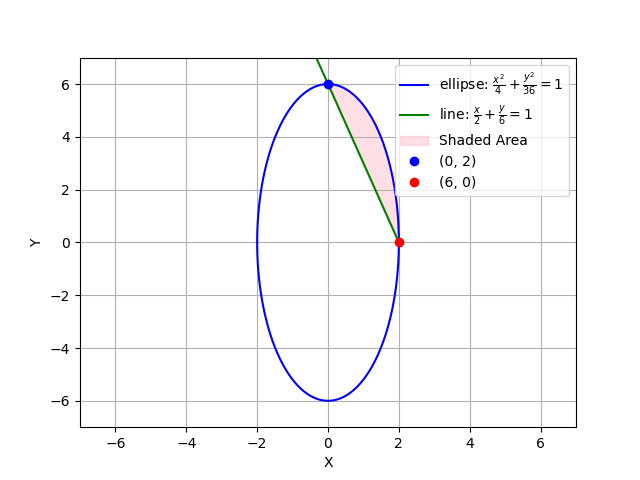
\includegraphics[width=0.7\columnwidth]{figs/fig.png}
    \caption{Area between line and ellipse}
\end{figure}
        \end{frame}
        \end{document} 
